\documentclass{report}

\usepackage[utf8]{inputenc} 		% Permet d'utiliser des sources LaTeX contenant des caractères accentués.
\usepackage[T1]{fontenc}				% Permet d'utiliser des sources LaTeX contenant des caractères accentués.
\usepackage[francais]{babel} 		% Permet de charger le package babel en lui indiquant que l'on veut travailler en français.
\usepackage[cyr]{aeguill} 			% Permet d'utiliser les guillemets français («»).
\usepackage{graphicx}           % Permet l'importation d'image.


\title{Améliorer la qualité des logiciels avec l'Intégration Continue}
\author{\textsc{Gaëtan Meynier}}
\date{\today}

\begin{document}

  \begin{titlepage}
    \centering
    {\scshape\LARGE Université Paris Dauphine \par}
    \vspace{1cm}
	  {\scshape\Large Mémoire de recherche\par}
    \vspace{0.5cm}
    Septembre 2016\par
    \vspace{4.5cm}
    {\huge\bfseries Améliorer la qualité des logiciels avec l'Intégration Continue\par}
    \vspace{2cm}
	  {\Large\itshape Gaëtan Meynier\par}
    \vspace{5cm}
	  \vfill
	    {\bfseries Supervisé par\par}
      \vspace{0.5cm}
	    Khalid \textsc{Belhajjame}, Maître de conférence à l'Université Paris Dauphine,
      Arthur \textsc{Szumovicz}, Consultant en système d'information à AXA.
	  \vfill
  \end{titlepage}

  \tableofcontents                % Table des matières.

  \chapter{Introduction}
  Depuis maintenant quelques années (il est difficile de donner une date précise), les DSI s’appuient sur la mouvance agile afin de mener à bien leurs projets. Aujourd’hui, les patterns agiles arrivent à maturité et offrent un éventail de méthodologies adaptables à tous les contextes. Les méthodes agiles garantissent la satisfaction du client et non la conformité aux termes d’un contrat de développement. Elles sont centrées sur la satisfaction de besoin du client et non sur les termes contractuels du projet. Nous n’allons pas aborder en profondeur le concept de l’agilité, ceci n’est pas le propos de ce mémoire, mais nous allons tout de même faire un petit rappel des idées fortes de cette méthodologie. Il faut des cycles courts, quelques semaines tout au plus, et découper le projet en petites tâches puis les hiérarchiser en fonction du besoin. Cela permet d’éviter le superflu et de se concentrer au début de chaque cycle sur ce qui a de la valeur pour l’utilisateur final. Le feedback permanent devient la règle d’or, avec des validations à chaque étape et des techniques ludiques d’évaluation de l’utilité des fonctions. L’agilité offre une meilleure visibilité et permet d’éviter les dérives observées lorsque les développeurs sont isolés. Le changement est autorisé voir encouragé, même tardivement,  car c’est un avantage décisif pour le client. Cela permet de ne pas se priver des bonnes idées en cours de route et surtout d’éliminer les mauvaises idées lancées au début du projet. Les méthodes agiles favorisent la co-construction, en intégrant l’annonceur lui-même dans le travail quotidien et en responsabilisant la totalité de l’équipe de développement, créant ainsi un véritable esprit collaboratif et l’ensemble du projet en gagne en qualité.\\

  Cependant l’agilité, lorsqu’elle est exclusivement cantonnée au développement, se trouve néanmoins freinée par les tâches d’exploitation. Le mouvement DevOps a pour objectif d’étendre les pratiques agilistes à la livraison et au déploiement du projet.

    \section{Motivation}

    \section{Scope}

    \section{Problèmes de recherche}

    \section{Methodes}

      \subsection{Méthodes de recherche}

      \subsection{Collecte de données}

    \section{Structure du mémoire}

  \chapter{DevOps}
  Le mouvement DevOps, contraction de « Development » et « Operational » tente de répondre à la problématique, certainement aussi ancienne que les DSI, qu’est la frontière qui sépare les développeurs (ceux qui écrivent le code source) et l’exploitation (ceux qui déploient et exploitent).\\

  \begin{figure}
    \begin{center}
      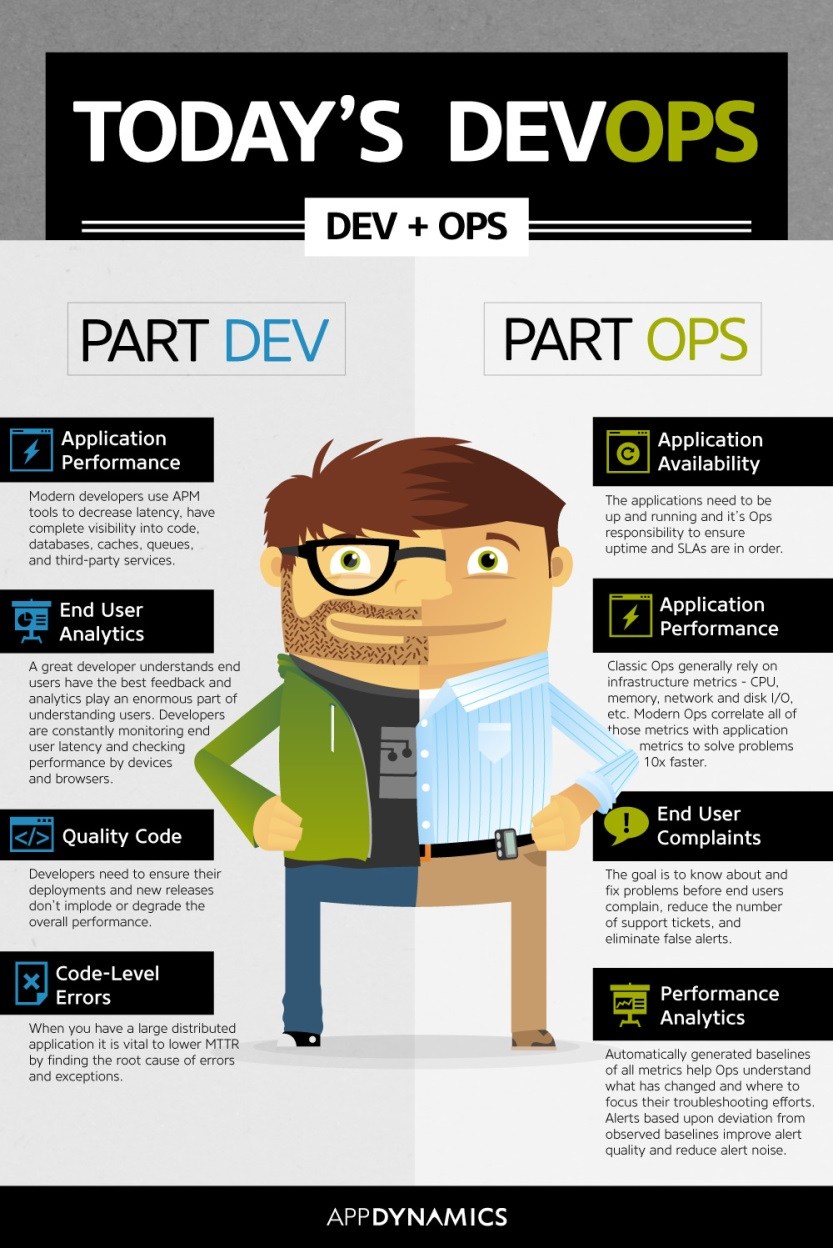
\includegraphics[scale=1.5]{images/devops.png}
    \end{center}
    \caption{DEV + OPS}
    \label{Devops}
  \end{figure}

  Les attentes et perspectives autour de Devops sont nombreuses :\\

  \begin{itemize}
    \item \textbf{Des cycles de déploiement plus courts} : les DevOps jouent un rôle clé dans la réduction du temps du cycle de déploiement des logiciels, passant de quelques semaines à seulement quelques heures, permettant une plus grande flexibilité quant aux nouvelles fonctionnalités et changements à apporter au produit initial.
    \item \textbf{Mise à disposition de nouveaux services plus rapidement} : des déploiements fréquents associés à des délais de livraison plus rapides permettent une agilité opérationnelle.
    \item \textbf{Une satisfaction client améliorée} : grâce à des applications ciblées et de qualité, conformes aux retours clients end to end.
    \item \textbf{Des coûts réduits} : L’automatisation permet aux équipes de réaffecter des ressources précieuses à des tâches à plus haute valeur.
    \item \textbf{Conformité et Gouvernance} : Automatisation du tracking et reporting end-to-end sur les phases de livraison/déploiement contenu.\\
  \end{itemize}

  \section{« The Wall of Confusion »}

  \section{La Culture}

  \section{« Infrastructure As Code »}

  http://blog.octo.com/et-si-devops-nous-emmenait-vers-tdi-test-driven-infrastructure/

  \section{Cloud Computing}

    \subsubsection{Définition}
    Il existe autant de réponse à « Qu’est-ce que le Cloud Comptine ? » que de distribution linux. J’ai pour ma part décider de baser mon analyse sur la définition fournit par NIST (National Institut of Standards and Technology):\\

    \begin{quotation}
      \emph{« Cloud Computing is a model for enabling ubiquitous, convenient,on-demand network access to a shared pool of configurable Computing resources (e.g., networks, servers, storage, applications, and services) that can be rapidly provisioned and released with minimal management effort or service provider interaction. This Cloud model is composed of five essential characteristics, three service models, and four deployment models. »}
    \end{quotation}

    \begin{quotation}
      \emph{« Le Cloud Computing est un modèle qui permet un accès omniprésent, pratique et à la demande à un réseau partagé et à un ensemble de ressources informatiques configurables (comme par exemple : des réseaux, des serveurs, du stockage, des applications et des services) qui peuvent être provisionnées et libérées avec un minimum d’administration. »}\\
    \end{quotation}

    Pour simplifier, le Cloud Computing est la dématérialisation de l’informatique. C’est le fait de déporter toutes les opérations normalement effectuées sur nos ordinateurs sur des ordinateurs distants, autrement dit sur internet. L’ensemble de ses serveurs constituent le Cloud (Voir Figure \ref{Cloud Computing}).

    \begin{figure}
      \begin{center}
        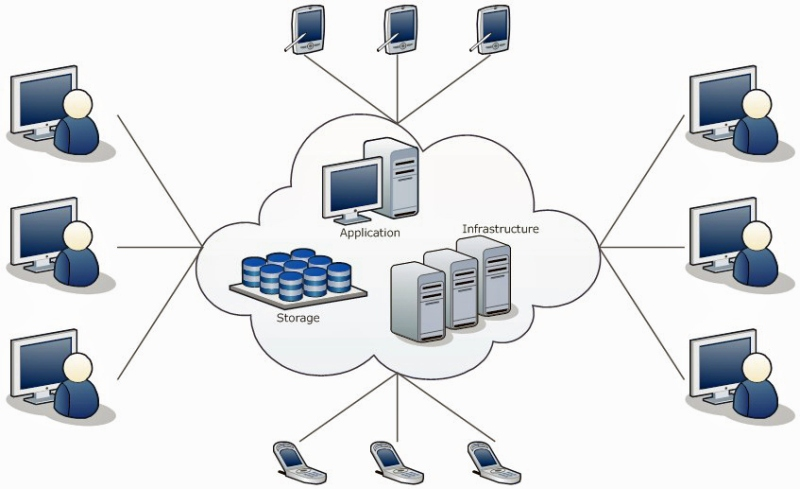
\includegraphics[scale=0.3]{images/CloudComputing.png}
      \end{center}
      \caption{Schématisation du Cloud Computing}
      \label{Cloud Computing}
    \end{figure}

    \subsubsection{Un service à la demande et une flexibilité des ressources.}
    Avec les applications Cloud, nous adaptons le flux de données à l'évolution de nos besoins: nous ne payons que pour ce que nous consommons. Et nous n'avons plus à nous soucier de manquer de capacité.

    \subsubsection{Accès universel par le réseau}
    Le terme de nuage représente bien le concept. Imaginons que nos ordinateurs nous suivent partout, que nous puissions y accéder n’importe où, n’importe quand depuis n’importe quel terminal. Imaginons un accès universel aux ressources stockés sur nos ordinateurs.

    \subsubsection{Une mise en commun des ressources}
    L'application de correctifs, la mise à niveau et le test d'applications peuvent occuper nos équipes informatique s plusieurs jours par mois. Grâce aux applications Cloud, cette problématique disparaît.\\

    Cependant ce n’est pas si simple que cela. Il existe trois types de Cloud: le Cloud public (loué par des prestataires), le Cloud privé (créer et gérer par notre entreprise) et le Cloud hybride (un mélange des deux précédents).

    \subsection{Le Cloud public}
    Le Cloud public appartient à des prestataires de service qui louent l’utilisation de leurs serveurs en facturant leur utilisation à la demande. Nous payons le flux de données échangé. Il dispose principalement de quatre modèles qui correspondent à des besoins bien distincts: le IAAS, le PASS, le SAAS et le STAAT.

      \subsubsection{Le Cloud IAAS ou Infrastructure As A Service (infrastructure en tant que service)}
      Le IAAS correspond à une infrastructure informatique (serveurs, réseaux, stockage) hébergé chez le prestataire de service. Nous n’avons pas besoin d’acheter le matériel nécessaire à notre infrastructure, nous nous contentons de la louer mais la gérons comme bon nous semble. Nous installons les serveurs que nous souhaitons utiliser et nous gérons l’ensemble des OS installés sur ces derniers. IAAS est utile si l’on désire créer ses propres plateformes pour ensuite y déployer des applications comme sur des serveurs locaux.

      \subsubsection{Le Cloud PAAS ou Plateform As A Service (plateforme en tant que service)}
      Le PAAS constitue l’utilisation par le biais d’internet de plateformes sur lesquelles nous pouvons déployer nos propres applications. C’est le niveau d’exécution des logiciels. Nous louons une plateforme, c’est à dire une machine avec un OS, le tout prêt à l’emploi.

      \subsubsection{Le Cloud SAAS ou Software As A Service (logiciel en tant que service)}
      Il s’agit d’utiliser des logiciels directement sur le Cloud, la plupart du temps via un navigateur web. Nous n’avons pas d’achat de licence, pas d’installation sur nos propres terminaux, pas d’entretiens. Le logiciel « tourne » sur des serveurs dans des datacenters (Voir Figure \ref{Google Cloud}).

      \begin{figure}
        \begin{center}
          
\includegraphics[scale=1]{images/googleDrive.png}
        \end{center}
        \caption{Exemple: la suite bureautique proposée par Google}
        \label{Google Cloud}
      \end{figure}

      \subsubsection{Le STAAT ou Storage As A Service (stockage en tant que service)}
      Le STAAT permet simplement des stocker nos données.

    \subsection{Le Cloud privé}
    Le Cloud privé est un Cloud propre à notre entreprise. A l’aide d’outils de virtualisation il est possible de transformer les serveurs existants au sein de l’entreprise. Cela créé un réseau puissant disponible, comme le Cloud public, à tout moment et à tout endroit mais géré entièrement par notre entreprise.

    \subsection{Las avantages du Cloud Computing}
    Les avantages du Cloud Computing sont nombreux. Si l’accessibilité est l’avantage le plus visible, il faut remarquer que l’utilisation du Cloud Computing permet à l’entreprise d’avoir une grande agilité, allant du démarrage rapide de son activité à un déploiement tout aussi rapide de nouvelles applications et donc un gain de temps et d’argent pour l’entreprise.\\

    De plus avec l’utilisation d’un Cloud public l’entreprise n’a plus d’investissement lourd en capital informatique, plus de dépendance en perte de temps et en entretient des infrastructures. Gains de places et de performances sont au rendez-vous.\\

    Cependant il faut soulever un petit bémol. En effet la contrepartie de tous cela est une dépendance totale envers internet et les prestataires de service. Ainsi qu’un coût croissant à mesure que les besoins de l’entreprises grandissent.

    \subsection{Quel Cloud choisir?}
    Si nous disposons déjà de serveurs et que nos besoins sont constants nous opterons pour le Cloud privé. Nous virtualiserons notre infrastructure et profiter de notre propre Cloud. Nos investissements sont ainsi préservés et nous gagnerions en productivité.\\

    En revanche, si nous ne disposons pas de serveurs ou que nous commençons tout juste notre activité et que nous ne souhaitons pas investir dans un parc informatique de serveur complet nous opterons pour un Cloud public. Economie et flexibilité sont au rendez-vous avec les services à la demande.\\

    Enfin si nous possédons des serveurs mais que notre activité fluctue beaucoup, nous demandant parfois des capacités plus fortes nous opterons pour le Cloud hybride. Nous concernerons ainsi notre autonomie avec notre Cloud privé et étendrons notre capacité ponctuellement avec le Cloud public.\\

    Pour conclure, si le Cloud Computing offre une grande disponibilité et une adaptabilité exemplaire, qui en font un service formidable, il n’en reste pas moins dépendant d’internet et les risques en matières de sécurité sont encore mal évalués.

  \chapter{Intégration Continue}

    \section{Histoire}
    Dans l’industrie logicielle l’intégration d’un projet logiciel est souvent un moment lourd et douloureux. La mise en commun des différents modules composants l’application entraine de grave problème d’intégration. Les modules fonctionnent correctement individuellement mais se confrontent à des problèmes de synergie. La résolution de ces problèmes demande un effort important qui s’accroisse avec la complexité du système. L’introduction des techniques et méthodologie de l’Intégration Continue, estompent les problèmes d’intégration jusqu’à les réduire en un non-évènement.\\

    \begin{quotation}
      \emph{« Continuous integration is the practice of making small well-defined changes to a project’s code base and getting immediate feedback to see whether the test suites still pass. »}
    \end{quotation}

    \begin{quotation}
      \emph{« L'intégration continue est la pratique de faire de petits changements bien définis à la base du code source d'un projet et d'obtenir une rétroaction immédiate pour voir si les suites de test passent toujours. »} Paul Duvall \cite{Duv07}.\\
    \end{quotation}

    L’idée d'Intégration Continue a été développée par la communauté Extreme Programming (XP) et a été décrit par Kent Beck dans son livre « Extreme programming explained » \cite{Bec99}, articulé autour de douze pratiques de développement agile. Son but étant de prévenir les problèmes décrit ci-dessus désignés comme « integration hell » (l’enfer de l’intégration) par Ron Jeffries en 2001. Martin Fowler a également été l'un des premiers contributeurs ayant écrit sur l’intégration continue \cite{Fow00}. Plus tard, les travaux ont été poursuivi par Paul Duvall qui a écrit tout un livre à propos de l’intégration \cite{Duv07}.

    Martin Fowler \cite{Fow00} désigne 10 principes clés pour réussir un Intégration Continue efficace :\\

    \begin{itemize}
      \item maintenir un référentiel de source unique,
      \item automatiser la construction de l’application (build),
      \item automatiser les tests,
      \item valider quotidiennement les modifications au niveau de la branche principale du contrôle de version (commit),
      \item créer une build d’intégration à chaque commit sur la branche principale,
      \item assurer une build rapide,
      \item effectuer les tests dans un environnement clone de la production,
      \item assurer la disponibilité pour tous des derniers livrables,
      \item assurer une visibilité pour tous,
      \item automatiser le déploiement.\\
    \end{itemize}

    \section{L'Intégration Continue comme un processus}
    L’Intégration Continue est un processus où le logiciel est construit à chaque changement. Cela signifie que lorsqu’une modification apportée par un développeur est détectée dans le code source, une construction automatique est déclenchée sur une machine de construction séparé. La construction contient plusieurs étapes prédéfinies comme la compilation, les tests, la génération de métrique du code source et le déploiement - entre autres. Une fois la construction terminé un rapport est envoyé aux membres du projet spécifié. Le rapport de compilation indique le résultat de chaque étape de la construction avec des informations détaillées sur les erreurs possibles qui ont pu survenir.\\\\

    Martin Fowler \cite{Fow00} décrit l’Intégration Continue comme :\\
    \begin{quotation}
      \emph{« Continuous Integration is a software development practice where members of a team integrate their work frequently, usually each person integrates at least daily - leading to multiple integrations per day. Each integration is verified by an automated build (including test) to detect integration errors as quickly as possible. Many teams find that this approach leads to significantly reduced integration problems and allows a team to develop cohesive software more rapidly. »}
    \end{quotation}

    \begin{quotation}
      \emph{« L'Intégration Continue est une pratique de développement logiciels où les membres d'une équipe intègre leur travail régulièrement, chaque développeur intègre au moins quotidienne une version - conduisant à de multiples intégrations journalière. Chaque intégration est vérifiée par une construction automatique (y compris le test) pour détecter les erreurs d'intégration le plus rapidement possible. De nombreuses équipes trouvent que cette approche conduit à réduire considérablement les problèmes d'intégration et permet une équipe pour développer des logiciels cohésifs plus rapidement. »}\\
    \end{quotation}

      \subsection{Les bénéfices de l’Intégration Continue}
      Selon Paul Duvall \cite{Duv07}, l'intégration logiciels n’est pas un problème dans les petites équipe, un à deux développeurs, mais quand le nombre de collaborateur se multiplie ou que diverses équipes commencent à travailler ensemble sur un projet, l'intégration logiciels devient un problème, car plusieurs personnes modifient simultanément des morceaux de code devant fonctionner ensemble. Vérifier que les divers composants logiciels interdépendants continuent de fonctionner correctement ensemble soulève la nécessité d'intégrer plus tôt et plus souvent. Les points suivants décrivent les différents effets bénéfiques que Paul Duvall a été en mesure d'identifier.

        \subsubsection{Réduire les risques}
        En intégrant plusieurs fois par jour, les risques de dysfonctionnement sont considérablement réduits. Les problèmes sont remontés dès leur intégration et peuvent même être la cause d’un rejet d’intégration. Ceci étant possible par l’intégration et l’exécution de tests et l’inspections automatiquement du code source après chaque modification.

        \subsubsection{Générer des logiciels déployables}
        L'un des objectifs du développement logiciel agile est de déployer tôt et souvent. L’Intégration Continue aide à atteindre cet objectif en automatisant les étapes de production des logiciels déployables. Des logiciels déployables et fonctionnels est l'avantage le plus évident de l’Intégration Continue du point de vue extérieur, car le client ou l'utilisateur final est généralement pas intéressés par le fait que l’Intégration Continue ait été utilisé dans le cadre de l'assurance qualité. Il est aussi l'atout le plus tangible, étant le résultat final de l’Intégration Continue.

        \subsubsection{Permettre une meilleure visibilité du projet}
        Le fait que le processus d’Intégration Continue s’exécute régulièrement fournit la capacité à remarquer les tendances et à prendre des décisions sur la base d’informations réelles. Sans Intégration Continue, les informations doivent être recueillies manuellement requérant du temps et des efforts. Le  processus d’Intégration Continue fourni en temps réel les informations sur l'état de la construction et de la qualité des dernières mesures tels que la couverture de test ou le nombre de codage violations de la convention.

        \subsubsection{Une plus grande confiance du produit}
        En ayant une Intégration Continue en place, l'équipe projet se protège contre certaines actions négatives portées aux codes sources. L’Intégration Continue agit comme un filet de sécurité, il repère les erreurs tôt et régulièrement. Ce qui se traduit par une plus grande confiance à l'équipe. Même des changements importants peuvent être faits avec confiance.

      \subsection{Le cycle de travail de l’Intégration Continue}
      Alors que l’Intégration Continue est généralement orchestrée par un serveur d’Intégration Continue, c’est aussi une façon de travailler. L'idée principale est d'intégrer les changements au code source aussi souvent qu’il y ait du nouveau code ajoutant de la valeur à l’application, à savoir plusieurs fois par jour. Cela rend l'intégration du code plus facile parce qu'il y a moins de code à intégrer à la fois. Il contribue également dans une situation où plusieurs personnes modifient la même base de code, car les développeurs auront ainsi les modifications apportées par d'autres.
      L'intégration des changements au code source de base comporte plusieurs étapes. Le cycle de travail est illustré dans le schéma suivant (Voir Figure \ref{IC workflow}). Il est basé sur les idées présentées par Martin Fowler \cite{Fow00} avec une phase de mise à jour supplémentaire, après l'exécution des tests. Cette phase de mise à jour est nécessaire dans la situation où le test prend du temps de sorte qu'il pourrait déjà y avoir de nouvelles modifications intégrées pendant notre phase de test.\\

      \begin{enumerate}
        \item récupérer le code source du référentiel (Check-out),
        \item modifier le code et créer les tests pour les modifications,
        \item vérifiez si quelqu'un d'autre a modifié le code source,
        \item exécuter tous les tests afin de vérifier que les modifications n’aient pas altéré le bon fonctionnement de l’application,
        \item vérifiez à nouveau si quelqu'un d'autre ont modifié le code source,
        \item valider les modifications dans le référentiel (Check-in),
        \item démarrer un nouveau cycle.\\
      \end{enumerate}

      \begin{figure}
        \begin{center}
          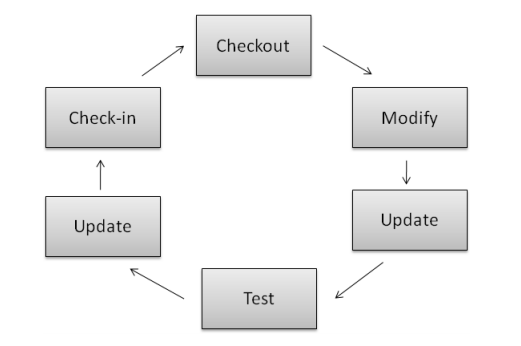
\includegraphics[scale=0.5]{images/ICWorkflow.png}
        \end{center}
        \caption{Cycle de travail de l’Intégration Continue}
        \label{IC workflow}
      \end{figure}

      Le cycle de travail commence créer une copie du code source hébergé sur le serveur de gestion de code qui est sur le point d'être modifié. Si le code avait précédemment récupéré, une mise à jour est faite à la place. Le développeur effectue les changements appropriés à sa tâche (nouvelle fonctionnalité, réfactorisation du code…) et implémente les tests appropriés afin de vérifier la conformité de son développement. Un test de développement vérifie que la sortie d’une méthode, en fonction de ses entrées, soit en adéquation avec le résultat attendu. Il est recommandé d’écrire les tests avant le code réel de l’application, ceci est appelé Test Driven Development (TDD).\\

      Dans un projet de logiciel, il est courant que de nombreux développeurs travaillent simultanément sur une même partie de code.  Par conséquent avant d’intégrer notre partie en code source, il est nécessaire de vérifier qu’aucune modification n’ait été faite par un développeur tierce sur par le biais d’une nouvelle mise à jour. Dans certains cas, il est possible que d’autres développeurs aient modifié exactement les mêmes lignes de code que nous produisant un ou plusieurs conflits. Dans ce cas, les conflits doivent être immédiatement résolus et tous les tests ré-effectués. Il est possible que dans cet intervalle une nouvelle version soit disponible sur le référentiel,  l'étape précédente doit être répétée jusqu'à ce qu'aucuns nouveaux changements ne soient détectés. Une fois cette synchronisation effectué le check-in peut être fait.

      \subsection{Comment l’Intégration Continue s’appuie-t-elle sur d’autres pratiques de développement}
      L’Intégration Continue comprend un ensemble de règles qui tous développeurs devraient suivre :

      \begin{enumerate}
        \item effectuer régulièrement des commits,
        \item ne pas commit des codes buggés,
        \item régler les problèmes et builder immédiatement,
        \item écrire des tests de développement automatisés,
        \item tous les tests et métriques doivent être valides,
        \item exécuter en local ses builds,
        \item éviter de travailler avec du code buggés.\\
      \end{enumerate}

      Ces règles ne sont pas nouvelles dans le monde du développement logiciel et sont aussi adopté d'autres pratiques de développement. Par conséquent, si des pratiques telles que les tests de développeur, les normes de codage, le refactoring et la propriété collective sont déjà mises en place au sein du projet, il est facile de commencer à utiliser l’Intégration Continue. Ces pratiques doivent être rigoureusement appliquées au travers de l’Intégration Continue sous peine d’empêcher les autres collaborateurs du projet de travailler. Prenons par exemple le cas d’un développeur ayant remanié une partie du code source et cassé quelques tests. Ne l’ayant pas remarqué, faute de n’avoir pas exécuté les tests, il valide ses changements dans le référentiel. La build éclate du faite que la règle « tous les tests doivent être au vert » n’est pas suivie. Maintenant si un autre développeur commence à travailler avec le code du référentiel, la première chose qu'il doit faire est de fixer ce qui avait été cassé par son collègue. Et cela peut prendre un beaucoup de temps, si cette personne ne connaît pas la partie de code qui provoque l’échec des tests.

    \section{L’Intégration Continue est un mélange de personnes et de systèmes}

      \subsection{Le développeur}
      !!!!!!!!!!!!!!!!! You build it, you run it !!!!!!!!!!!!!!!!!

      Pratiquer l’Intégration Continue exige de la discipline de la part des développeurs. Ils devront appliquer avec rigueur les pratiques de développement vus précédemment. Une fois le développement de la tâche effectué, le développeur doit exécuter une build sur sa propre machine de développement. On appelle cela une build privée. Cette étape permet de vérifier que les modifications apportées n’ont pas endommagé l'intégration avec le reste du code source. Il est important d'exécuter la build privée avant de valider les changements dans le référentiel de contrôle de version, car soumettre un code erroné peut empêcher les autres développeurs de travailler. Une fois l’exécution de la build privée avec succès, le développeur peut valider les modifications, et les tests. Si l'intégration de la build échoue malgré ses précautions, réparer cette build est la priorité numéro un.

      \subsection{Le référentiel de contrôle de version}
      L'intégration continue ne peut pas se faire sans référentiel de contrôle de version. Le référentiel de contrôle de version, également connu sous le nom de gestionnaire de code source (SCM), est un système utilisé pour stocker le code source et d'autres aspects du logiciel (comme la documentation) de manière centralisée. Il assure également le suivi de l'historique des versions et modifications effectuées au cours du développement. Les développeurs de logiciels ont la possibilité de revenir à une version antérieure ou la révision d'un logiciel, ou de prendre connaissances des changements apportés sur toute révision donnée. Ce référentiel fournit un point d'accès unique au code source pour les développeurs et le système d’Intégration Continue. Il peut être constitué de différentes branches du logiciel stocké. Une branche peut être créée pour la réécriture majeure d’un morceau de code ou pour le prototypage d’une idée intéressante qui pourrait ne pas se retrouver dans le produit final. La build d’intégration est exécuté sur la branche principale du référentiel de contrôle de version \cite{Duv07}. « Master » est la branche de code source où la plupart de la mise au point a lieu. Certains systèmes de contrôle de version appellent cela aussi « tunk » ou « head ». La ligne principale se doit d’être toujours stable et la build d’intégration ne doit jamais échouée quand elle est intégrée au référentiel.

      \begin{figure}
        \begin{center}
          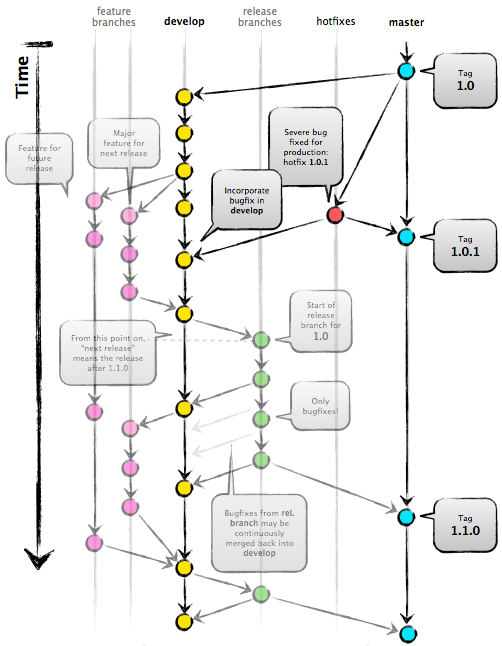
\includegraphics[scale=0.5]{images/gitFlow.png}
        \end{center}
        \caption{Ligne de temps d'un référentiel de contrôle de version}
      \end{figure}

      \subsection{Le serveur d’Intégration Continue}
      Le serveur d’Intégration Continue est l'orchestrateur de l'ensemble du processus. Il exécute la build d'intégration lorsqu'une modification a été apportée au référentiel. Quatre approches sont à prendre en compte.\\

      La première est la configuration d’un « post commit hook » au niveau du gestionnaire de code source. Le référentiel de contrôle de version peut-alors avertir immédiatement le serveur d’Intégration Continue qu’une modification a été ajoutée et validée. De cette façon une build d’intégration est exécutée pour chaque commit.\\

      Une autre approche, dénommée « polling approach »  \cite{Duv07} est de vérifier les changements à intervalles réguliers (de l’ordre de la minute). De ce fait plusieurs changements peuvent être effectués entre chaque build.\\

      Une troisième option est d’exécuter une build d’intégration à intervalles réguliers, mais si l'intervalle est trop long le bénéfice de la rétroaction est rapidement perdu.\\

      La quatrième et dernière option, consiste à intégrer une copie du référentiel principal, accessible uniquement par le serveur d’Intégration Continue, au niveau du serveur lui-même \ref{IC server}. Les développeurs n’ont ainsi accès qu’au référentiel du serveur d’Intégration Continue. Ce dernier peut alors être configuré afin de rejeter les modifications apporté au référentiel ne respectant pas les tests ou les métriques qualités prédéfinies. Garantissant ainsi la qualité de l’application.\\\\

      \begin{figure}
        \begin{center}
          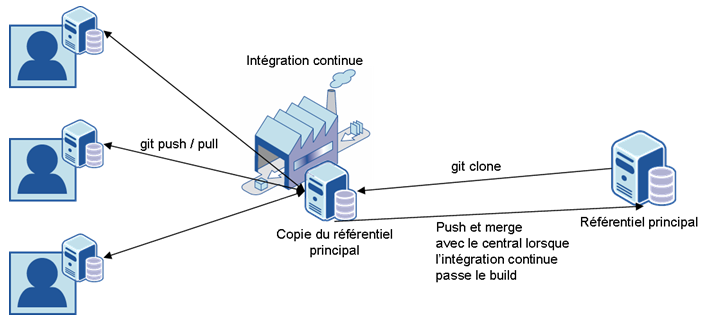
\includegraphics[scale=0.5]{images/ICServer.png}
        \end{center}
        \caption{Organisation d'un serveur d'Intégration Continue}
        \label{IC server}
      \end{figure}

      Le serveur d’Intégration Continue fournit également une vue, généralement une page web, qui expose l'état de santé de tous les « build jobs »\footnote{Build jobs : cela correspond aux différentes tâches du processus de build.} et afficher leurs résultats en temps réel  configurés (Voir Figure \ref{Jenkins build jobs}). Ce tableau de bord peut être affiché, par exemple, sur un grand écran dans la salle de l'équipe de développement pour donner un aperçu rapide et en temps réel des tâches effectués sur le serveur et voir ainsi s'il y a des constructions en cours d'exécution. De nombreux serveurs d’Intégration Continue proposent également un type de visualisation basé sur les principes des feux de circulation ou de météo de connaitre l’état des builds d’Intégration.\\

      Toutes les fonctionnalités d’un serveur d’Intégration Continue ne sont pas nécessaires pour faire de l’Intégration Continue. De nombreux scripts personnalisés peuvent effectuer les mêmes tâches, mais avoir un serveur conçu à cet effet aide beaucoup \cite{Duv07}. De plus en plus de solutions propriétaires ou open source\footnote{Open source : logiciel libre redistribution, d'accès au code source et de création de travaux dérivés.}  performe le marché et offre un environnement d’Intégration Continue stable et complet.\\

      Dans sa forme la plus simple, l’Intégration Continue pourrait être mise en place avec un seul ordinateur dédié exécutant des scripts afin de vérifier le code source du référentiel, lancer une build d’Intégration et envoyer des rapports une fois la build terminée. Le serveur d’Intégration Continue offre une autre possibilité en fournissant une interface utilisateur afin de configurer les multiples « build jobs ».

      \begin{figure}
        \begin{center}
          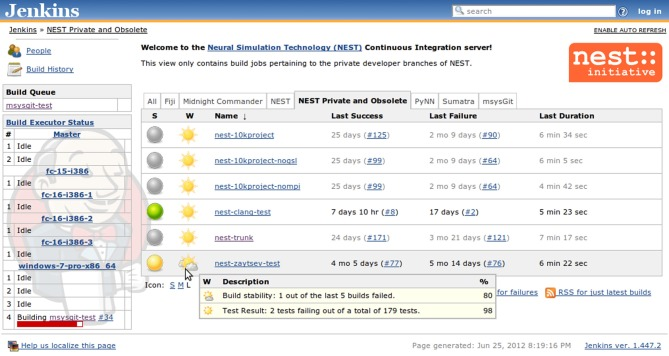
\includegraphics[scale=0.5]{images/jenkinsBuildJobs.png}
        \end{center}
        \caption{Tableau de bord d'un serveur d'Intégration Continue Jenkins}
        \label{Jenkins build jobs}
      \end{figure}

      \subsection{Les scripts de construction (build)}
      Généralement la plupart des étapes d’une build sont définies en utilisant un script de compilation. Un script de compilation peut être constitué d'un ou plusieurs scripts et il est utilisé, par exemple, pour compiler, tester, contrôler et déployer des logiciels. Toutes les mesures qui peuvent être automatisées pour construire et déployer des logiciels doivent être automatisées. Cela économise du temps et les nerfs des développeurs. Il existe de nombreuses techniques disponibles comme Ant (Java), Make (C/C++) ou Scons (Python).\\

      Certains développeurs utilisent leur environnement de développement intégré (IDE) pour builder leurs logiciels. Dans ce cas la build ne pourra être encadré par l’Intégration Continue. L’intégration Continue nécessite que la build puisse être exécutée indépendamment de tout IDE \cite{Duv07}.


      \subsection{Les mécanismes de feedback}
      Lorsque la build d'intégration est terminée, les résultats doivent être accessibles dès que possible. La capacité à fournir un feedback rapide est l'un des avantages de l’Intégration Continue. La rétroaction est disponible immédiatement une fois la build terminée. La rétroaction peut être diffusée par différent canaux ; tableau de bord, courrier électronique, flux RSS. En cas de build défectueuse, la réparation peut démarrer immédiatement après réception de l'avis.\\

      Certain pionnier commence même à intégrer le terme de « monitoring continue » dans l’ingénierie logicielle en complément de l’Intégration Continue. Le monitoring continu consiste à avoir un affichage visible par tous les membres de l’équipe de développement, actualisé en temps réel, donnant un feedback direct sur l’état des différentes builds simplifié et directement interprétable. Cet affichage est dans la plupart du temps un moniteur, mais d’autres solutions plus amusantes, telles que la lampe à lave ou une « ambient orb » commencent à s’imposer \cite{Swa04}.


      \subsection{Les machines de build d’intégration}
      Un serveur d’Intégration Continue à besoin d'un hôte pour fonctionner. La machine de build d’intégration (ou nœud)  est une machine distincte qui doit imiter l'environnement de production. Si possible, elle doit fonctionner avec le même système d'exploitation, la même version de serveur de base de données et les mêmes versions de librairies doivent être utilisées, comme il est prévu pour en production. Chaque différence augmente le risque des tests de ne pas détecter les problèmes liés à l’environnement de la production \cite{Fow06}.\\

      Dans le cas où de nombreux « build jobs » sont configurés pour l’application, pour réduire la durée de la build et ainsi augmenté la rapidité de la rétroaction il peut être nécessaire de paralléliser les tâches sur plusieurs machines (scalabilité horizontal). Certains logiciels de serveur d’Intégration Continue fournissent une architecture maître-esclave qui permet ainsi de diviser la charge de travail sur plusieurs hôtes.\\

      Parfois plusieurs environnements sont nécessaires pour builder sur différentes plates-formes. La virtualisation des serveurs apportent la réponse à ce problème. En utilisant une infrastructure de virtualisation bien établis, il est assez facile d’exécuter des instances esclaves multiples sur un seul nœud physique. Ces instances pouvant fonctionner sous différents systèmes d’exploitation. Certains logiciels de serveur d’Intégration Continue offre la possibilité à la build d’intégration de fonctionner simultanément sur ces différentes instances et de collecter les résultats pour chaque environnement.\\

      Puis virtualisation est quelque chose de valeur à l'aide de la peine de la virtualisation diminue \cite{Bar03}. Certains logiciels de serveur de CI comme Hudson permet même de construction de travail afin de fonctionner simultanément sur plusieurs serveurs virtuels et de collecter des résultats pour chaque environnement.


    \section{Caractéristique de l’Intégration Continue}
    Selon Paul Duvall \cite{Duv07} seules quatre caractéristiques sont nécessaires à l’Intégration Continue :\\
    \begin{itemize}
      \item une connexion à un référentiel de contrôle de version,
      \item un script de compilation,
      \item un mécanisme de rétroaction,
      \item un processus pour intégrer les modifications au code source (manuelles ou serveur d’Intégration Continue).\\
    \end{itemize}

    Ces éléments seuls sont nécessaires à la construction d’un système d’Intégration Continue efficace, qui est expliqué plus en détail dans les sections suivantes.


      \subsection{Compilation du code source}
      La compilation du code source est l'une des caractéristiques de base du système d’Intégration Continue. La compilation crée des exécutables binaires à partir de source lisible (pour les développeurs). Lors de l'utilisation des langages dynamiques comme Python ou Ruby la compilation est différente. Les binaires ne sont pas compilés, à la place les développeurs ont la possibilité d'effectuer un checking strict, qui peut être considéré comme de la compilation dans le contexte de ces langues \cite{Duv07}.

      \subsection{Tests}
      Les tests sont la partie la plus vitale de l’Intégration Continue. Beaucoup considèrent qu’une Intégration Continue sans automatisation du contrôle continu ne peut être un Contrôle Continue \cite{Duv07}. Il est difficile d'avoir confiance dans les changements du code source sans une bonne couverture de test. Les tests peuvent être automatisés en utilisant des outils de tests unitaires tels que JUnit (Java), NUnit (C\#), ou d'autres framework\footnote{Framework : ensemble d'outils et de composants logiciles.} de xUnit. Certains de ces frameworks peuvent également générer des rapports machines lisibles, qui peuvent être analysés et utilisés pour générer des représentations graphiques telles que des pages Web ou des tableaux (Voir Figure \ref{xUnit output}).

      \begin{figure}
        \begin{center}
          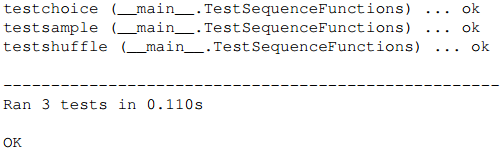
\includegraphics[scale=0.8]{images/tests.png}
        \end{center}
        \caption{xUnit output}
        \label{xUnit output}
      \end{figure}

        \subsubsection{Niveaux de tests}
        Le test peut être effectué à différents niveaux \ref{Testing levels}. Le plus bas niveau de test est appelé test unitaire. Une unité est la plus petite partie d’une application testable. Cela correspond une fonction ou une méthode dans une classe. Le but des tests unitaires est de vérifier que les différentes parties du code fonctionnent comme elles le devraient. Ils assurent la stabilité du code en testant chaque unité unitairement. Les régressions seront ainsi remontées très rapidement ce qui permet de manipuler le code source avec confiance. Les tests unitaires sont généralement écrits par le développeur qui a également écrit le code. Une bonne pratique des tests unitaires est de commencer par écrire les tests et d’ensuite les valider par le code. C’est ce qu’on appelle le « Tests Driven Development » (TDD) ou Développement Dirigé par les Tests ».\\

        Le niveau suivant est le test d'intégration. Dans ce contexte d’Intégration nous devons vérifier que les modules individuels du logiciel fonctionnent aussi en tant que groupe.\\

        \begin{quotation}
          \emph{« Le test d'intégration identifie les problèmes qui se produisent lors de la combinaison d'unités. En utilisant un plan de test exigeant que vous testiez chaque unité et que vous vérifiez la viabilité de chacune d'elles avant de les combiner, vous savez que les erreurs découvertes lors de la combinaison d'unités concernent probablement l'interface entre les unités. Cette méthode réduit le nombre de possibilités à un niveau beaucoup plus simple d'analyse. »} Microsoft \cite{Mic16}.\\
        \end{quotation}

        Le troisième niveau teste les API d’un point de vue externe, sans se préoccuper de fonctionnement interne du système. Le test système analyse le flux de retour de l’API en fonction de son flux d’entrée afin  de détecter les défauts à la fois dans les inter-assemblages mais également au sein du système dans son ensemble. Cette méthode est appelé « boîte noire ».\\

	       Le test fonctionnel est le quatrième niveau de test majeur. Il assure la stabilité de l’application en reproduisant le parcours d’un utilisateur sur le navigateur. Il teste le bon fonctionnement de l’application et remontent les régressions fonctionnelles.\\

         D’autres niveaux de test existent, tel que le test applicatif qui assure la sécurité et la compatibilité, le test d’IHM qui fiabilise l’ergonomie et la visibilité, le test de charge qui veille à la performance et à la robustesse de l’application...

         \begin{figure}
           \begin{center}
             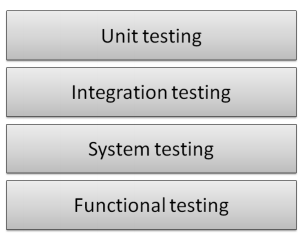
\includegraphics[scale=0.7]{images/testingLevels.png}
           \end{center}
           \caption{Les principaux niveaux de test}
           \label{Testing levels}
         \end{figure}

        \subsubsection{Exécuter les tests plus rapides en première}
        Lorsque le logiciel se développe le nombre de tests augmente, ce qui se traduit par une hausse du temps d’exécution des tests leur de la build d’intégration. Si l’ensemble des tests est exécuté en une seule fois cela peut prendre du temps et ainsi faire perdre le bénéfice de rétroaction rapide. Pour faire face à ce syndrome, les tests doivent être classés de plus rapides au plus lents en terme d’exécution. Les tests peuvent aussi être divisés en plusieurs étapes. Les rapports seront envoyés à la fin de chaque étape garantissant un feedback rapide.\\

        Les tests unitaires nécessitent peu de temps à mettre en place et sont les tests les plus rapides à exécuter. L’exécution d’un test unitaire ne doit pas excéder la fraction de seconde. Ces tests sont exécutés de nombreuses fois par jour par développeurs. La rapidité d’exécution est primordiale sinon les tests deviennent une méthodologie de développement à éviter ce qui est contraire au principe de l’Intégration Continue \cite{Duv07}. Les tests unitaires sont donc de bons candidats pour être exécuter au cours de la première étape.\\

        La configuration des tests d'intégration et des tests système nécessitent beaucoup plus de temps que celle des tests unitaires. La mise en place la (des) base(s) de données avec des données de test et de lancement réel de l’application sont des tâches relativement chronophages. L’exécution de ces tests peut être une étape longue. Les tests d’intégration et système peuvent être exécutées dans des étapes ultérieures ou à des intervalles périodiques. Par exemple nous pouvons exécuter une suite complète de tests de plusieurs heures tous les soirs. Nous appelons ce processus Daily Build \cite{McC96}.

        \subsubsection{Ecrire des tests d’échecs}
        L’écrire et l’exécution automatique des tests avec l’Intégration Continue diminue la fréquence des logiciels défectueux. Mais l’Intégration Continue n’est pas infaillible \cite{Duv07}. Si un défaut est trouvé, il doit être immédiatement fixé et pour éviter qu’elle se reproduise, un test défectueux devra être implémenté. L'idée sous-jacente est d’améliorer continuellement la qualité de l’application.

      \subsection{Qualimétrie}

      \subsection{Base de données d’intégration}
      L’Intégration Continue ne se limite pas à la construction du code source, elle peut également être utilisée dans le développement de base de données. Les bases de données sont des parties intégrantes des applications et ont donc besoin d’être intégré dans le processus d’Intégration Continue. La création d’une base de données fonctionnelle lors d’une build d’intégration nécessite un ensemble de scripts stocké dans le référentiel de contrôle de version. Ces scripts comprennent les définitions des tables, les procédures stockées, le partitionnement... L’exécution des tests fonctionnels nécessite des données « réelles » afin de garantir un environnement proche de la production. Des scripts de « données », exécuter après la création de la base de données complètent la mise en place d’une base de données fonctionnelle.\\

      Par exemple, lorsqu’un développeur ou un administrateur de base de données (DBA) apporte une modification à script de base de données et le valide au niveau du système de contrôle de version (check-in), la build d’intégration (la même que celle utilisée pour l’intégration du code source) construit la nouvelle base de données et lance les tests.

      \subsubsection{Test unitaire sur les fonctions de base de données}
      Pour des raisons de sécurités et de performances les fonctions propres aux bases de données sont stockées et exécutées par elles-mêmes. On les appelle alors « procédures stockées ». Comme pour les méthodes de l’application les procédures doivent être testées et automatisées par des scripts qui seront exécutés lors de la build d’intégration.

      \subsection{Inspection Continue}
      Le code source peut être examiné manuellement et/ou automatiquement. La revue de code manuelle peut être effectuée selon deux principes, le « pair programming » (écriture du code en binôme) ou le « code review » (session collective de relecture du code). Elle améliore la qualité algorithmique et syntaxique du code source de l’application et permet aux développeurs d’échanger sur les bonnes pratiques. Pour une revue de code automatique, de nombreux analyseurs de code statique sont disponibles selon les langages de développement. Ces outils analysent les fichiers sources dans le but de souligner les violations de règles prédéfinies propre au langage et d’améliorer la syntaxe de nos lignes de code.\\

      La différence entre la revue de code manuelle faite par des humains et la revue de code automatique  faite par des outils d’analyses est double. Exécuter les analyseurs  de code statique est peu cher et une fois automatisé ils garantissent une relative propreté au code source. De plus un ordinateur est toujours objectif et ne se lasse pas d’inspecter l’intégralité du code à chaque fois qu’un changement est engagé dans le référentiel de contrôle de version.\\

      Les analyses statiques de code automatisé sont efficientes pour des grandes bases de code. Elles permettent aux développeurs de se concentrer sur les parties importantes. Elles offrent des métriques de qualité sous la forme de rapport d’inspection après chaque exécution. Les revues automatisées ne remplacent pas les revues manuelles, elles permettent de recentrer l’intelligence humaine là où elle est nécessaire.\\

      De nombreux IDE (environnement de développement intégré) intègrent des fonctionnalités d’inspection pour aider les développeurs dès l’écriture du code avec une mise en forme automatisée, la mise en évidence des variables non utilisées, l’utilisation illégale de certain élément… Il est fortement encouragé de les utiliser mais ne remplace en aucun cas les revues de code.\\

      Il existe également des outils qui proposent de réécrire certain bout de code selon une convention particulière, de détecter les blocs de code en double…


        \subsubsection{Différences entre inspection et test}
        Le test (vu précédemment) est dynamique et exécute l’application, ou un fragment de l’application, pour tester les fonctionnalités. L’inspection, quant à elle, analyse le code selon un ensemble de règles prédéfinies. Les deux sont des concepts similaires dans le sens ou aucun ne modifient le code source, ils ne font que remonter les problèmes résidant dans l’application.

        \subsubsection{Rapport d’inspection}
        Les outils d’analyse statique de code fournissent un grand nombre de mesures et de rapports, encore faut-il les interpréter. Depuis quelques décennies des chercheurs étudient ces mesures afin de trouver une corrélation entre les défauts soulignés par les analyses et le code source.\\

        Une des principales mesures étudiée est la complexité cyclomatique, qui quantifie la complexité du code source en comptant le nombre de chemins distincts au travers d'un programme représenté sous la forme d'un graphe \cite{Kan03}. Les analystes suggèrent une complexité de 10 car plus grand est ce nombre, plus important sera le risque de défauts \cite{Wat96}. Le moyen le plus efficace pour réduire la complexité cyclomatique d’une application est d'appliquer la technique de la méthode d'extraction et de distribuer la complexité en petits méthodes, plus faciles à gérer, et donc plus testable, \cite{Duv07}.\\

        Outre les problèmes de complexités les rapports d’inspection nous fournissent des mesures sur des problèmes liés à l’architecture de notre application ; « l’afferent coupling » et « l’efferent coupling ». Ces métriques comptent les nombres de dépendances vers, où à partir d’un objet soulignant ainsi les risques de responsabilités ou de dépendances trop fortes. Elles permettent de déterminer le niveau de risque dans le maintien et l’évolutivité du code. Duvall introduit l'utilisation de ces deux valeurs combinées pour calculer une valeur d'instabilité.\\

        \begin{center}
            $Instability=\frac{EfferentCoupling}{EfferentCoupling + AfferentCoupling}$\\
        \end{center}

        La compréhension de ces mesures et de l'analyse des rapports d'inspection peut une réelle plus-value sur le temps investi. Les problèmes de maintenabilité peuvent être repérés dès le début et les risques de défauts peuvent être réduits.


    \section{Déploiement Continue}
    L'un des objectifs de l’Intégration Continue est d'avoir un logiciel prêt et fonctionnel pour le déploiement à tout moment du développement. Toutes les étapes vues précédemment sont des parties du processus de déploiement visant à générer les artefacts de logiciels fournis avec les dernières modifications de code disponibles dans un environnement de test \cite{Duv07}. Une fois l’application packagée il est possible de l'installer automatiquement sur les serveurs de production avec le Déploiement Continue. Pour cela, nous avons six étapes de haut niveau:\\
    \begin{itemize}
      \item étiqueter les actifs d'un référentiel,
      \item produire un environnement propre, exempt d'hypothèses,
      \item générer et étiqueter une version directement à partir du référentiel et l'installer sur la machine cible,
      \item effectuer les tests avec succès à tous les niveaux dans un clone de l'environnement de production,
      \item créer des rapports de rétroaction de build,
      \item	si nécessaire, la release peut être annulée en utilisant des étiquettes dans le système de contrôle de version.\\
    \end{itemize}

      \subsection{Les bonnes pratiques du Déploiement Continue}

        \subsubsection{Etiqueter les actifs d’un référentiel}

        \subsubsection{Produire un environnement propre}

        \subsubsection{Etiqueter chaque build}

        \subsubsection{Exécuter tous les tests}

        \subsubsection{Créer des build feedback reports}

        \subsubsection{Capacité à effectuer un rollback}

      \subsection{La dockerisation}
      Le site officiel de Docker définit son outils comme tel:\\

      \begin{quotation}
        \emph{« Docker est un outil qui peut empaqueter une application et ses dépendances dans un conteneur virtuel, qui pourra être exécuté sur n’importe quel serveur Linux »}\\
      \end{quotation}

      Le mot clé de cette définition est conteneur. Qu’est ce qu’un conteneur?

        \subsubsection{Le conteneur}
        Le conteneur n’est pas une notion nouvelle, ce n’est pas une notion inventé par Docker. Linux a un système de conteneur qui s’appelle LXC (LinuX Container) qui permet de gérer cet empaquetage.\\

        Un conteneur est globalement une sorte de boite, un peu comme une machine virtuelle, qui va être complètement isoler du système d’exploitation dans laquelle nous allons pouvoir installer toutes les librairies dont a besoin notre application pour fonctionner ainsi que notre application. Le conteneur étant complètement isolé du reste nous allons pouvoir la distribuer un peu partout, indépendamment du système d’exploitation.

        \subsubsection{Les avantages}
        Actuellement nos applications ont besoin de plus en plus de technologies pour fonctionner. Prenons un cas concret avec une application PHP.\\

        Une application PHP a besoin d’une certaine version de PHP, d’images magiques (pour la conversion d’images), d’une base de données, d’un système de cache, d’un serveur web (Nginx ou Apache), d’un indexeur (Elasticsearch)… Pour au final nous retrouver avec une application nécessitant de nombreuses dépendances.\\

        Le problème est que lorsque nous travaillons avec un administrateur système ou un hébergeur tier le déploiement de notre application peut rapidement s’avérer fastidieuse. Ces derniers devront installer sur chaque serveur de déploiement les dépendances requises pour le bon fonctionnement de notre application. En tant que développeur nous ne sommes pas forcément sensible à toutes les problématiques liées aux serveurs ce qui créé un climat hostile entre les développeurs et les administrateurs systèmes.\\

        Le gros avantage du conteneur est que ce dernier va pouvoir être livré avec l’intégralité des dépendances liées à notre application.

        \subsubsection{Conteneur VS Machine virtuelle (VM)}
        Ce que nous venons de décrire est exactement le principe de fonctionnement d’une VM. Pour comprendre la différence entre ces deux technologies voici un petit schéma issu du site officiel de Docker (Voir Figure \ref{Virtual Machine}).\\

        \begin{figure}
          \begin{center}
            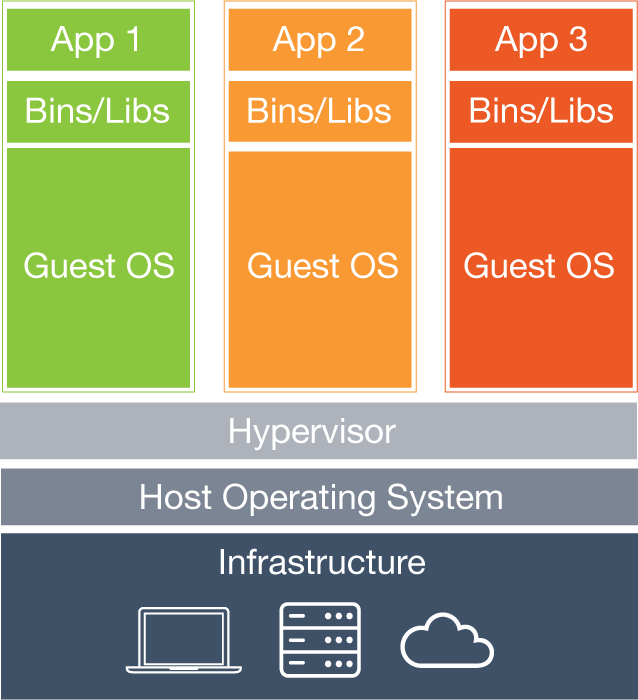
\includegraphics[scale=0.2]{images/virtualMachine.png}
          \end{center}
          \caption{Schéma de fonctionnement d'une machine virtuelle}
          \label{Virtual Machine}
        \end{figure}

        Voici la structure actuelle d’un serveur que l’on a avec des machines virtuelles. Nous nous retrouvons avec une infrastructure et par dessus un système d’exploitation qui va ensuite faire fonctionner diverses machines virtuelles. Pour schématiser nous avons un ordinateur dans un ordinateur. Le problème de cette structure est la redondance des système d’exploitation. Si notre serveur héberge x machine(s) virtuelle(s), nous aurons x système(s) d’exploitation(s) installer sur notre serveur, ce qui consomme beaucoup de ressources mémoires et processeurs.\\

        Le système de conteneur nous permet de nous absoudre de cette contrainte et te faire fonctionner nos application directement sur le système d’exploitation du serveur hôte. Nous avons ainsi plus besoin de virtualiser les différents systèmes d’exploitations de nos applications. Ce qui va alléger notre structure serveur (Voir Figure \ref{Container}).\\

        \begin{figure}
          \begin{center}
            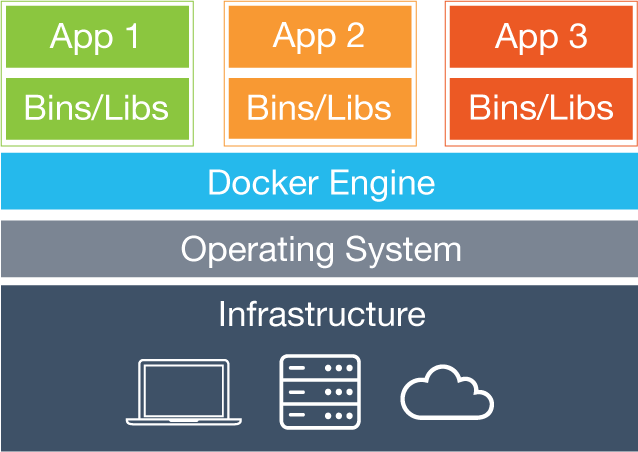
\includegraphics[scale=0.2]{images/container.png}
          \end{center}
          \caption{Schéma de fonctionnement d'un conteneur}
          \label{Container}
        \end{figure}

        \subsubsection{Les avantages}
        Les avantages de l’utilisation de conteneur sont nombreux. Nous allons nous intéressez aux quatre principaux, les gains en performance, la probabilité des conteneurs, leur scalabilité et les facilités de déploiement.\\

        Un système d’exploitation s’appuie sur de nombreux processus coûteux en mémoire et en CPU (temps de calcul d’un ordinateur). La réduction du nombre de systèmes d’exploitation à un unique OS tournant sur notre serveur hôte augmente considérablement les performance de ce dernier.\\

        Le système de boite isolée rend la technologie des conteneurs beaucoup plus portable. Si nous voulons transférer une machine virtuelle d’un serveur A à un serveur B nous devons effectuer un snapshot intégral de notre 1 VM et le transférer. Le problème est qu’une machine virtuelle pèse lourd. Du coup le transfert d’une VM prendre beaucoup de temps.\\

        Le troisième avantage du conteneur est qu’il est beaucoup plus facilement scalable. Nous allons pouvoir bouger nos petits boîtes très rapidement d’un serveur à l’autre, et même les faire évoluer en terme de performance.\\

        Le dernier avantage que nous allons abordé est lié à la faculté de portable et scalable de nos conteneurs est le déploiement de ces derniers. Déployer un conteneur va être très simple. Vu qu’un conteneur est léger et qu’il embarque l’intégralité des dépendances nécessaires au bon fonctionnement de notre application nous allons pouvoir envoyer à notre administrateur système ou notre hébergeur l’intégralité de notre environnement de production.

      \subsection{La « bêta perpétuelle »}
      Le principe de la « bêta perpétuelle » a été introduit pour la première fois par Tim O’Reilly dans le manifeste du Web 2.0, qui expose le principe selon lequel:\\
      \begin{quotation}
        \emph{« Les utilisateurs doivent être considérés comme des co-développeurs, en suivant les principes Open Source (…). Avec le Web 2.0, ce principe évolue vers une position plus radicale, la bêta perpétuelle, dans laquelle le produit est développé de manière ouverte, avec de nouvelles fonctionnalités offertes sur une base mensuelle, hebdomadaire, ou même quotidienne. »}\\
      \end{quotation}

      Le terme « bêta perpétuelle » désigne le fait que notre application n’est jamais finalisée. Elle s’absout des contraintes habituelles liées au cycle de développement en « release » au profit d’une livraison en continu des nouvelles fonctionnalités.

        \subsubsection{Release early, release often}
        Derrière ce nouveau concept se cache un concept déjà bien en place chez les agilistes (du point de vue de l’itération courte) et dans le monde de l’Open Source (du point de vue de la récolte continue du feedback), le « Release early, release often », traduit en français par « Publiez tôt, publiez souvent ». Cette pratique a été décrite par Eric Steven Raymond dans “La cathédrale et le bazar” où il formulait explicitement:\\
        \begin{quotation}
          \emph{« Publiez tôt. Publiez souvent. Et écoutez vos clients »}\\
        \end{quotation}

        Cette méthodologie vise à réduire les temps de développement et améliorer l’implication de l’utilisateur dans la conception du logiciel afin de créer un produit correspondant à ces attentes et ainsi éviter la création d’un logiciel que personne n’utilisera.

        \subsubsection{Les services en ligne (Software As A Service)}
        Le concept de « bêta perpétuelle » a été rendu possible grâce au Cloud Computing et plus particulièrement à la généralisation du service en ligne ou « Software As A Service ». L’hébergement de l’application par l’éditeur permet d’absoudre ce dernier au traditionnel cycle de déploiement d’un logiciel et de ne gérer qu’une seule version de son application. Les services en ligne sont continuellement mise à jour sans pour autant en informer l’utilisateur. Les nouvelles fonctionnalités, découverte au fur et à mesure par l’utilisateur, permettent un apprentissage progressif des nouveautés applicatives.

        \subsubsection{La « Customer driven roadmap »}
        L’hébergement de l’application sur serveur offre à l’éditeur une maîtrise total de sa plateforme de production. Il peut ainsi mettre en place des sondes analytiques afin de récolter des informations sur l’usage de notre application et l’accueil réservé à nos nouvelles fonctionnalités par l’utilisateur.

        \subsubsection{Les pré-requis}
        La mise en place d’une stratégie de « bêta perpétuelle » requiert certains pré-requis pour en garantir le succès:\\
        \begin{itemize}
          \item une intégration continu,
          \item une livraison continue,
          \item un déploiement continu,
          \item une stratégie de type « One click deployment / Rollback » pour une restauration rapide de l’application au dernier état stable.\\
        \end{itemize}

        \subsubsection{Conclusion}
        Le concept de la « bêta perpétuelle » est présent chez de nombreux géants du Web tel que Google, Facebook, Amazon, Twitter, Flickr… Peu en font mention dû à la mauvaise image du terme « bêta », qui pour la conscience collective, se réfère à un produit non fini et peu fiable. Prenons en exemple Gmail, la boite aux lettres mails développé par Google, qui jusqu’en 2009 intégrait la mention « bêta » dans son logo. De petites fonctionnalités unitaires sont fréquemment proposés aux utilisateurs. En fonction de leur niveau d’adoption Google les intègrent ou non à la version standard de son service.

        \subsection{Le « Zero Downtime Deployment »}
        Nous avons vu précédement comment améliorer le «Time To Market » tout en garantissant la qualité des développements. L'étape suivante est de garantir que ces déploiements de plus en plus fréquents n'impactent pas la disponibilité de l'application. Le « Zero Downtime Deployment » (ZDD) offre une approche qui permet de déployer une nouvelle version issus de la build sans interrumption de service. Pou cela le ZDD repose sur trois grands patterns, le « Blue/Green Deployment », le « Canary Release » et le « Dark Launch ».
          \subsubsection{Les patterns}
          Le « Blue/Green Deployment » est le pattern de base du ZDD. L’application, hébergée sur au moins deux chaines applicatives, déploie sa version N+1 sur une des chaînes (ou plusieurs) tandis que le service en ligne est maintenu en version N sur les autres chaines applicatives (Voir Figure \ref{BlueGreen}).\\

          \begin{figure}
            \begin{center}
              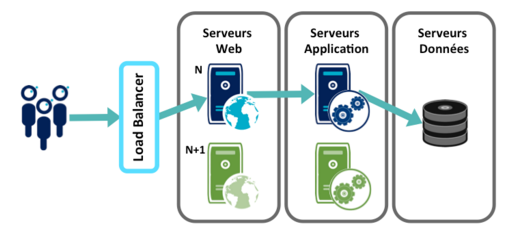
\includegraphics[scale=0.7]{images/BlueGreenDeployment.png}
            \end{center}
            \caption{Schéma de pattern « Blue/Green Deployment »}
            \label{BlueGreen}
          \end{figure}

          Une fois le déploiement effectué, notre nouvelle version doit être testé par une population restreinte d’utilisateurs. Le « Canary Release » confronte la version N+1 à une niche d’utilisateurs cibles tandis que la version N reste accessible à la majorité des utilisateurs (Voir Figure \ref{CanaryRelease}).\\

          \begin{figure}
            \begin{center}
              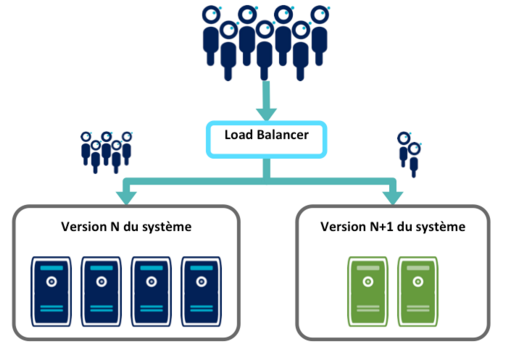
\includegraphics[scale=0.6]{images/CanaryRelease.png}
            \end{center}
            \caption{« Schéma de pattern Canary Release »}
            \label{CanaryRelease}
          \end{figure}

          La dernière étape du ZDD est le test de charge de notre nouvelle application. Le « Dark Launch » stimule progressivement le traffic généré par l’utilisateur afin de valider les performances et la scalabilité de notre plateforme. La stimulation progressive du traffic permet de préparer et d’optimiser au mieux notre plateforme afin que la mise en production finale de notre application se déroule sans problème.

          \subsubsection{La mise en oeuvre}
          Load balancer\\

          Les sessions\\

          La modification du schéma de base de données\\

        \subsection{Le « Flipping feature »}

    \chapter{Etude de l'art}

      \section{Logiciel en développement}

      \section{Processus de développement logiciel}

        \subsection{Scrum dans l'AgilLab}

        \subsection{Comment l’Intégration Continue s’intègre-t-elle dans le processus de développement logiciel}

        \subsection{Les équipes de développement}

      \section{La sécurité à l'esprit}

    \chapter{Implémentation}

      \section{Choisir ses outils}

        \subsection{Scaling}

        \subsection{Le choix du serveur d’Intégration Continue}
          \subsubsection{Support du langage de programmation}

          \subsubsection{Support du Source Code Management}

          \subsubsection{Gestion des builds}

          \subsubsection{Sécurité}

          \subsubsection{Autres caractéristiques}

          \subsubsection{Extensibilité}

          \subsubsection{Installation et configuration}

          \subsubsection{Autres questions à examiner}

      \section{Logiciels et outils utilisés}

        \subsection{Serveur d’Intégration Continue}

        \subsection{Logiciel de gestion de configuration}

        \subsection{Outils de build}

        \subsection{Automatisation des tests et de la couverture de code}

        \subsection{Documentation Continue}

        \subsection{Déploiement Continue}

        \subsection{Feedback Continue}

      \section{Architecture}

        \subsection{Serveur d’Intégration Continue}

        \subsection{Logiciel de gestion de configuration}

        \subsection{Réseaux et déploiement}

      \section{Configuration}

        \subsection{« Build jobs »}

          \subsubsection{Découpage des jobs}

          \subsubsection{Etablir des relations}

        \subsection{Reporting}

      \section{Délivrables et artéfacts de build}

  \listoffigures                  % Liste les figures
  \bibliographystyle{alpha}       % les trois premières lettres du nom de l'auteur accolées aux deux derniers chiffres de l'année de parution
  \bibliography{MemoireM2}        % mon fichier de base de données s'appelle MemoireM2.bib
\end{document}
